
%
% NIM Paper Sync
%
\documentclass[preprint,12pt]{elsarticle}

%% Use the option review to obtain double line spacing
%% \documentclass[authoryear,preprint,review,12pt]{elsarticle}

%% Use the options 1p,twocolumn; 3p; 3p,twocolumn; 5p; or 5p,twocolumn
%% for a journal layout:
%% \documentclass[final,1p,times]{elsarticle}
%% \documentclass[final,1p,times,twocolumn]{elsarticle}
%% \documentclass[final,3p,times]{elsarticle}
%% \documentclass[final,3p,times,twocolumn]{elsarticle}
%% \documentclass[final,5p,times]{elsarticle}
%% \documentclass[final,5p,times,twocolumn]{elsarticle}

%% For including figures, graphicx.sty has been loaded in
%% elsarticle.cls. If you prefer /to use the old commands
\usepackage{epsfig}
\usepackage{subcaption}

%% The amssymb package provides various useful mathematical symbols
\usepackage{amssymb}
\usepackage{xcolor}
%% The amsthm package provides extended theorem environments
%% \usepackage{amsthm}

%% The lineno packages adds line numbers. Start line numbering with
%% \begin{linenumbers}, end it with \end{linenumbers}. Or switch it on
%% for the whole article with \linenumbers.
%% \usepackage{lineno}

\journal{Nuclear Instruments and Methods}

\begin{document}

\begin{frontmatter}

%% Title, authors and addresses

%% use the tnoteref command within \title for footnotes;
%% use the tnotetext command for theassociated footnote;
%% use the fnref command within \author or \address for footnotes;
%% use the fntext command for theassociated footnote;
%% use the corref command within \author for corresponding author footnotes;
%% use the cortext command for theassociated footnote;
%% use the ead command for the email address,
%% and the form \ead[url] for the home page:
%% \title{Title\tnoteref{label1}}
%% \tnotetext[label1]{}
%% \author{Name\corref{cor1}\fnref{label2}}
%% \ead{email address}
%% \ead[url]{home page}
%% \fntext[label2]{}
%% \cortext[cor1]{}
%% \address{Address\fnref{label3}}
%% \fntext[label3]{}

\title{Boiling Study for H, H2, H3 and He3 Targets}
%\title{Performance of the Hall A Tritium Target}

\author[Kent]{Sheren Alsalmi}
\author[UNH]{Nathaly Santiesteban}
\author[UNH]{Shujie Li}
\author[JLab]{David Meekins}

\address[Kent]{Kent State University}
\address[UNH]{University of New Hampshire}
\address[JLab]{Jefferson Lab}

\begin{abstract}
When the beam passes through a cryo-target, the local temperature fluctuations could 
cause a variation in the target density. This density variation is called \emph{Boiling}, 
and it increases with increasing current. The density fluctuation due to passing beam, 
or the boiling effect, for jlab Tritium experiments has been studied for Hydrogen (H), 
Deuterium (H2), Tritium (H3) and Helium (He3) targets.\par
\end{abstract}

\begin{keyword}
%% keywords here, in the form: keyword \sep keyword

%% PACS codes here, in the form: \PACS code \sep code
%% MSC codes here, in the form: \MSC code \sep code
%% or \MSC[2008] code \sep code (2000 is the default)
\end{keyword}
\end{frontmatter}

%% \linenumbers

%% main text
\section{Introduction}
\label{}
%%%%%

\section{Method Overview}
One way to study the boiling effect is by using the \textbf{Yield Analysis}, where the charge normalized yield is calculated versus current. A decrease in the charged normalized yield at higher currents, indicates that the target's density is decreasing. In another words, the target is \emph{boiling}. \par
\textbf{\underline{Steps for Yield Analysis:}}
\begin{enumerate}
\item{At each current, the total charge is calculated using:
\begin{equation}\label{eq:charge}
Q = a\times \Delta Counts + b\times \Delta Time
\end{equation}
wheren $Q$ is the total charge, $a$ and $b$ are the slop and offset identified by calibrating the Beam Charge Monitors "BCM's" frequency $vs.$ unser current . One can get the $Counts$ and $Time$ from the BCM and Clock scalers respectively. For this study, the dnew BCM is used, and the calibration constants are: $a=0.0003264$ and $b=0.1055$ (see Fig.\ref{fig:dnew})}
\begin{figure}[htb]
\centering
 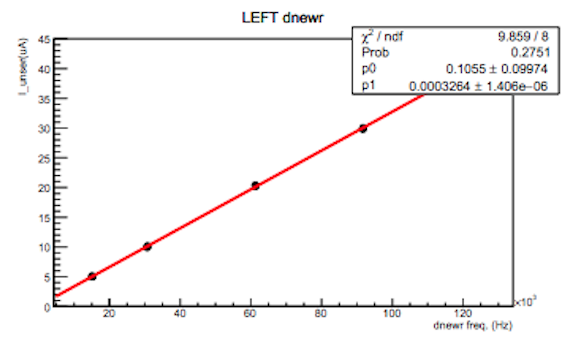
\includegraphics[width=0.7\linewidth]{dnew.png}
  \caption{dnew Calibration by: Nathaly Santiesteban}
  \label{fig:dnew}
\end{figure}
\item{The charge yield of a current $I$, $Yield(I)$, is then calculated using the following:
\begin{equation}\label{eq:y}
Yield(I) = \frac{N_{good}\times PS}{Q\times efficiencies \times LT}
\end{equation}
where $N_{good}$ is the number of good electrons at each current. Determining $N_{good}$,\emph{i.e.} selecting good electrons, is discussed in the following sections. PS and LT are the pre-scale and live-time of each run respectively. The $efficiencies$ include both detectors and trigger efficiencies.}
\item{The charge normalized yield is calculated by normalizing the charge yield for a current $I$, eq.\ref{eq:y}, over the charge yield when there is no current.
\begin{equation}
Y_{norm}(I) = \frac{Yield(I)}{Yield(I=0)}
\end{equation}
Since we don't really know what the charge yield should be at zero current, we use the charge yield at the lowest current available (2.5 $\mu$A for this study) as a normalization factor. Then fit the results so that the normalized yield will be equal to 1 at $I=0$. 

}
\end{enumerate}
\section{Electron Selection:}
  In order to extract a good electron sample, several cuts were applied on the recorded data:
 


Type your introduction here.

Example reference to the Hall A NIM paper~\cite{Alcorn:2004sb}.

%% The Appendices part is started with the command \appendix;
%% appendix sections are then done as normal sections
\appendix
\section{Acknowledgments}
%% \label{}

\bibliographystyle{elsarticle-num} 
\bibliography{references.bib}

\end{document}
\endinput
%%
%% End of file `elsarticle-template-num.tex'.
